%%% LaTeX Template: Article/Thesis/etc. with colored headings and special fonts
%%%
%%% Source: http://www.howtotex.com/
%%%
%%% Modified Oct 2021 by CDM
%%% Restructured 2026 by CDM to follow ISO/IEC/IEEE 29148:2018 (Requirements engineering)

%%%  Preamble
\documentclass[11pt,letterpaper]{article}
\usepackage[margin=1.0in]{geometry}
\usepackage[T1]{fontenc}
\usepackage[bitstream-charter]{mathdesign}
\usepackage[latin1]{inputenc}
\usepackage{amsmath}
\usepackage{xcolor}
\usepackage{cite}
\usepackage{hyphenat}
\usepackage{graphicx}
\usepackage{float}
\usepackage{subfigure}
\usepackage{sectsty}
\usepackage[compact]{titlesec}
\usepackage[tablegrid]{vhistory}
\usepackage{pbox}
\usepackage{longtable}
\allsectionsfont{\color{accentcolor}\scshape\selectfont}

%%% Definitions
\definecolor{accentcolor}{rgb}{0.0,0.0,0.5}
\newcommand{\teamname}{Team Name}
\newcommand{\productname}{Product Name}
\newcommand{\coursename}{CSE 4316: Senior Design I}
\newcommand{\semester}{Fall 2026}
\newcommand{\docname}{System Requirements Specification}
\newcommand{\department}{Department of Computer Science \& Engineering}
\newcommand{\university}{The University of Texas at Arlington}
\newcommand{\authors}{Alan Turing \\ Grace Hopper \\ John Von Neumann \\ Ada Lovelace \\ Charles Babbage}

%%% Headers and footers
\usepackage{fancyhdr}
	\pagestyle{fancy}						% Enabling the custom headers/footers
\usepackage{lastpage}
	% Header (empty)
	\lhead{}
	\chead{}
	\rhead{}
	% Footer
	\lfoot{\footnotesize \teamname \ - \semester}
	\cfoot{}
	\rfoot{\footnotesize page \thepage\ of \pageref{LastPage}}	% "Page 1 of 2"
	\renewcommand{\headrulewidth}{0.0pt}
	\renewcommand{\footrulewidth}{0.4pt}

%%% Change the abstract environment
\usepackage[runin]{abstract}			% runin option for a run-in title
\abslabeldelim{\quad}
\setlength{\abstitleskip}{-10pt}
\renewcommand{\abstractname}{}
\renewcommand{\abstracttextfont}{\color{accentcolor} \small \slshape}	% slanted text

%%% Start of the document
\begin{document}

%%% Cover sheet
{\centering \huge \color{accentcolor} \sc \textbf{\department \\ \university} \par}
\vspace{1 in}
{\centering \huge \color{accentcolor} \sc \textbf{\docname \\ \coursename \\ \semester} \par}
\vspace{0.5 in}
\begin{figure}[h!]
	\centering
   	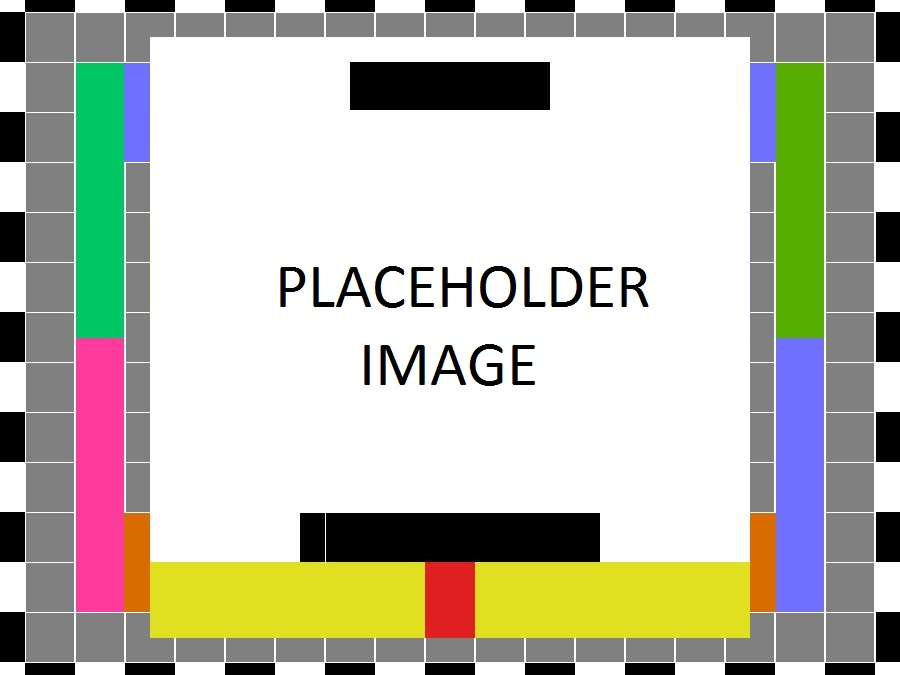
\includegraphics[width=0.60\textwidth]{images/test_image}
\end{figure}
\vspace{0.5 in}
{\centering \huge \color{accentcolor} \sc \textbf{\teamname \\ \productname} \par}
\vspace{0.5 in}
{\centering \large \sc \textbf{\authors} \par}
\newpage

%%% Revision History
\begin{versionhistory}
  	\vhEntry{0.1}{10.01.2026}{GH}{document creation}
  	\vhEntry{0.2}{10.05.2026}{AT|GH}{complete draft}
  	\vhEntry{0.3}{10.12.2026}{AT|GH}{release candidate 1}
  	\vhEntry{1.0}{10.20.2026}{AT|GH|CB}{official release}
  	\vhEntry{1.1}{10.31.2026}{AL}{added customer change requests}
\end{versionhistory}
\newpage

%%% Table of contents
\setcounter{tocdepth}{3}
\tableofcontents
\newpage

%%% List of figures and tables (optional)
\listoffigures
\listoftables
\newpage

%%% NOTE TO STUDENTS (remove before submission):
%%% This template is organized to follow the System Requirements Specification (SRS)
%%% information item defined in ISO/IEC/IEEE 29148:2018, which supersedes the
%%% withdrawn IEEE Std 830-1998. Section 1 provides context, Section 2 defines the
%%% requirements engineering conventions used, and Sections 3-11 contain the
%%% requirements themselves grouped by type. Section 12 addresses verification and
%%% traceability, and Section 13 lists deferred (Future) requirements.

\section{Introduction}
This System Requirements Specification (SRS) describes the requirements for the \productname\ system. It is organized in accordance with the SRS information item defined in ISO/IEC/IEEE 29148:2018 \cite{ISO29148}, the current international standard for requirements engineering (which supersedes the withdrawn IEEE Std 830-1998). Replace this paragraph with a one-paragraph synopsis of the product and the purpose of this document.

\subsection{Purpose}
State the purpose of this SRS and identify the intended readership (customer, sponsor, team members, instructors, future maintainers). Explain that this document is the authoritative, agreed baseline of what the system shall do and shall not do, and that requirements in it may not be changed without agreement of the intended customer/sponsor.

\subsection{Scope}
Name the software/system product(s) to be produced. Explain what the product will and will not do, and describe the application and benefits of the product. Be careful to bound the scope: describe the boundary between this system and the external systems, users, and environment it interacts with.

\subsection{Product Overview}
Provide the context needed to understand the requirements that follow. Per ISO/IEC/IEEE 29148, address at least the four topics below.

\subsubsection{Product Perspective}
Describe how this product relates to other products or systems. Is it self-contained, a component of a larger system, or a replacement for an existing system? Include a high-level context diagram showing the system boundary, its users, and the external systems/interfaces it connects to.

\begin{figure}[h!]
	\centering
   	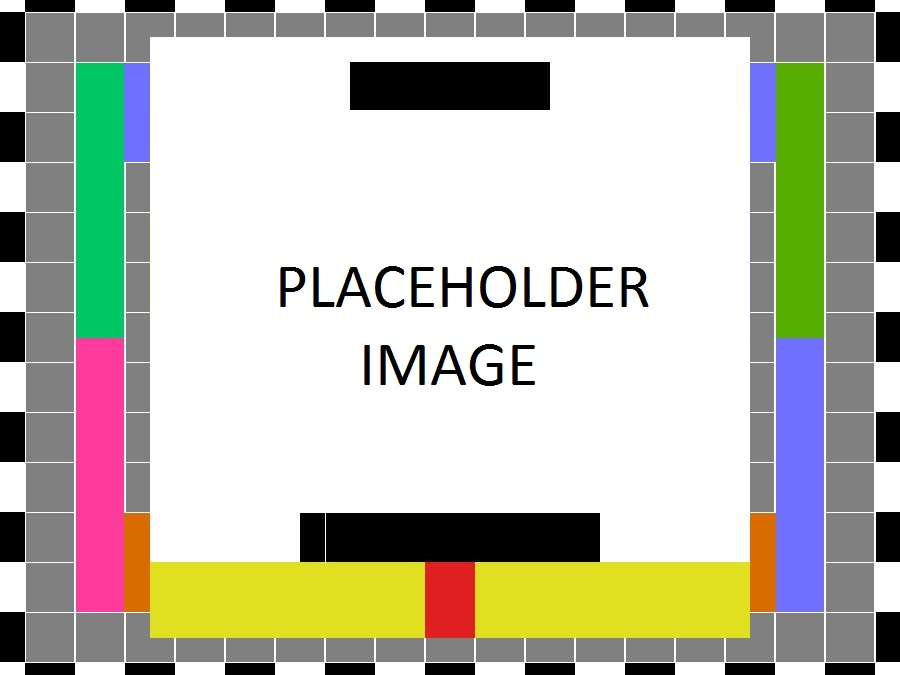
\includegraphics[width=0.60\textwidth]{images/test_image}
    \caption{\productname\ system context diagram}
\end{figure}

\subsubsection{Product Functions}
Summarize, at a high level, the major functions the product will perform. A bulleted list or a simple functional decomposition diagram is appropriate. Detailed, individually numbered requirements are specified in Sections 3--11; this subsection is only an orientation.

\subsubsection{User Characteristics}
Identify each class of user (end user, administrator, maintainer, external system) and the characteristics that affect requirements: expertise level, frequency of use, physical or accessibility considerations, and any assumptions about training.

\subsubsection{Assumptions \& Dependencies}
List the factors that, if changed, would change the requirements in this document. Distinguish assumptions (believed true but not guaranteed) from dependencies (relationships on external deliverables, systems, or organizations). Keep detailed project assumptions in the Project Charter; here, list only those that directly shape requirements.

\subsection{Definitions, Acronyms, and Abbreviations}
Define all terms, acronyms, and abbreviations required to interpret this document. A two-column table works well.

\begin{table}[H]
\caption{Definitions, acronyms, and abbreviations}
\begin{center}
    \begin{tabular}{ | p{3cm} | p{10cm} |}
    \hline
    \textbf{Term} & \textbf{Definition} \\ \hline
    SRS & System Requirements Specification \\ \hline
    Term & Definition of the term as used in this document \\ \hline
    \end{tabular}
\end{center}
\end{table}

\newpage
\section{Requirements Engineering Approach}
This section defines the conventions used to write and manage the requirements in this document. Remove the explanatory paragraphs from your final draft, but retain the tables and conventions your team adopts.

\subsection{Requirement Identification \& Numbering}
Every requirement in this document has a unique, persistent identifier so that it can be traced through design, implementation, and test. This template uses the scheme \texttt{[TYPE]-[NN]}, where \texttt{TYPE} denotes the requirement category and \texttt{NN} is a zero-padded sequence number, e.g. \texttt{FR-01} (functional), \texttt{PE-03} (performance), \texttt{SE-02} (security). Identifiers are never reused or renumbered once assigned; a retired requirement is marked \textit{deprecated} rather than deleted.

\begin{table}[H]
\caption{Requirement type prefixes}
\begin{center}
    \begin{tabular}{ | p{2cm} | p{11cm} |}
    \hline
    \textbf{Prefix} & \textbf{Requirement type} \\ \hline
    EI & External interface \\ \hline
    FR & Functional \\ \hline
    US & Usability \\ \hline
    PE & Performance \\ \hline
    PK & Packaging \& deployment \\ \hline
    SA & Safety \\ \hline
    SE & Security \& privacy \\ \hline
    MS & Maintenance \& support \\ \hline
    QA & Other quality attribute \\ \hline
    \end{tabular}
\end{center}
\end{table}

\subsection{Requirement Attributes}
Each requirement is specified using the attribute set below, adapted from the requirement attributes recommended in ISO/IEC/IEEE 29148:2018 \cite{ISO29148}. Every requirement in Sections 3--11 provides each of these attributes.

\begin{itemize}
  \item \textbf{Description} --- A single, testable statement of the required capability or characteristic, written using ``shall.''
  \item \textbf{Rationale} --- Why the requirement exists and the benefit it provides; this justifies the requirement and aids future change decisions.
  \item \textbf{Source} --- The origin of the requirement (customer, sponsor, named team member, regulation, standard, CSE Senior Design specifications, etc.).
  \item \textbf{Priority} --- The relative importance of the requirement (see below).
  \item \textbf{Verification Method} --- How conformance will be demonstrated (see below).
  \item \textbf{Constraints} --- Realistic constraints relevant to the requirement (economic, environmental, social, political, ethical, health \& safety, manufacturability, sustainability), as applicable.
  \item \textbf{Applicable Standards} --- Any specific standards that govern the requirement.
\end{itemize}

\subsection{Priority Scheme}
\begin{itemize}
\item \textbf{Critical} --- must have, or the product is a failure
\item \textbf{High} --- very important to customer acceptance and desirability
\item \textbf{Moderate} --- should have for proper product functionality
\item \textbf{Low} --- nice to have; will include if time/resources permit
\item \textbf{Future} --- not feasible in this version; recorded for a future release (see Section~13)
\end{itemize}

\subsection{Verification Methods}
Each requirement declares how it will be verified, using one of the four standard methods. The Verification \& Traceability section (Section~12) collects these into a requirements verification matrix.
\begin{itemize}
\item \textbf{Inspection (I)} --- verification by visual examination of the item or its documentation.
\item \textbf{Analysis (A)} --- verification by technical evaluation, modeling, or calculation.
\item \textbf{Demonstration (D)} --- verification by exercising the system and observing behavior, without detailed measurement.
\item \textbf{Test (T)} --- verification by controlled execution against defined inputs with measured, recorded results.
\end{itemize}

\subsection{Characteristics of Well-Formed Requirements}
Requirements in this document are written to satisfy the characteristics defined in ISO/IEC/IEEE 29148:2018: each requirement should be \textit{necessary, appropriate, unambiguous, complete, singular, feasible, verifiable, correct,} and \textit{conforming}, and the requirement set as a whole should be \textit{complete, consistent, feasible, comprehensible,} and \textit{able to be validated}. Avoid implementation detail unless it is a genuine constraint; specify \textit{what} is required, not \textit{how} it is built (design decisions belong in the Architectural and Detailed Design Specifications).

\newpage
\section{External Interface Requirements}
Include a header paragraph specific to your product here. External interface requirements define the interactions between the system and everything outside its boundary: users, hardware, other software, and communications. Per ISO/IEC/IEEE 29148:2018, specify each interface's content and format precisely enough that an independent team could implement either side. Where helpful, summarize the data crossing an interface in a table (name, description, direction, units/format, range).

\subsection{EI-01: [Interface Name]}
\subsubsection{Description}
The system shall \ldots\ (a single testable statement describing the interface, e.g. \textit{``The system shall expose a REST API over HTTPS accepting JSON request bodies encoded in UTF-8.''}). Identify whether the interface is a user interface, hardware interface, software interface, or communications interface, and reference the relevant data elements.

\begin{table}[H]
\caption{EI-01 data elements}
\begin{center}
    \begin{tabular}{ | p{2.5cm} | p{5cm} | p{2cm} | p{3cm} |}
    \hline
    \textbf{Element} & \textbf{Description} & \textbf{Direction} & \textbf{Format / Units} \\ \hline
    element 1 & description & in & type, range \\ \hline
    element 2 & description & out & type, range \\ \hline
    \end{tabular}
\end{center}
\end{table}
\subsubsection{Rationale}
Why this interface is required and the benefit it provides.
\subsubsection{Source}
Customer, sponsor, named team member, standard, etc.
\subsubsection{Priority}
Critical / High / Moderate / Low / Future
\subsubsection{Verification Method}
Inspection / Analysis / Demonstration / Test
\subsubsection{Constraints}
Any realistic constraints applicable to this interface.
\subsubsection{Applicable Standards}
e.g. IETF RFC 8259 (JSON), USB 2.0, IEEE 802.11, etc.

\subsection{EI-02: [Interface Name]}
Repeat the attribute block for each external interface.

\newpage
\section{Functional Requirements}
Include a header paragraph specific to your product here. Functional requirements are the directly observable features and functions of the product encountered by its users --- the ``look and feel'' and behavior that each end user should expect the product to do and/or not do. These correspond to the customer-facing requirements agreed with the intended customer/user/sponsor, and must not be changed without their specific agreement. Each requirement below is written as a singular, verifiable ``shall'' statement and carries the attribute set defined in Section~2.

\subsection{FR-01: [Requirement Name]}
\subsubsection{Description}
A detailed, singular, and verifiable statement of the feature/function. For example: \textit{The GUI background shall be slate blue (\#007FFF, six-digit hexadecimal), so that the GUI matches other software products offered by the customer.} It is acceptable and advisable to include drawings/graphics if they aid understanding.
\subsubsection{Rationale}
The customer need or benefit that this requirement satisfies. This justifies the requirement and supports future change decisions.
\subsubsection{Source}
The origin of the requirement (customer, sponsor, named team member, federal regulation, CSE Senior Design project specifications, etc.).
\subsubsection{Priority}
Critical / High / Moderate / Low / Future
\subsubsection{Verification Method}
Inspection / Analysis / Demonstration / Test --- how conformance will be shown.
\subsubsection{Constraints}
Realistic constraints relevant to this requirement (economic, environmental, social, political, ethical, health \& safety, manufacturability, sustainability), as appropriate.
\subsubsection{Applicable Standards}
Any specific standards that apply (e.g. a color specification, a data-format RFC, an accessibility guideline). Research and document which standards will be followed.

\subsection{FR-02: [Requirement Name]}
Repeat the attribute block for each functional requirement.

\newpage
\section{Usability Requirements}
Include a header paragraph specific to your product here. Usability requirements specify measurable objectives for how effectively, efficiently, and satisfactorily identified users can achieve their goals (see the quality model of ISO/IEC 25010:2023 \cite{ISO25010}). Prefer measurable targets --- learnability, task completion time, error rate, accessibility conformance --- over subjective language.

\subsection{US-01: [Requirement Name]}
\subsubsection{Description}
A measurable usability statement, e.g. \textit{A first-time user shall complete the primary task within 3 minutes without written instructions in at least 8 of 10 usability trials.}
\subsubsection{Rationale}
Why this level of usability matters to the customer or end users.
\subsubsection{Source}
Source of the requirement.
\subsubsection{Priority}
Critical / High / Moderate / Low / Future
\subsubsection{Verification Method}
Typically Demonstration or Test (e.g. moderated usability sessions, accessibility audit).
\subsubsection{Constraints}
Applicable constraints (accessibility mandates, device limitations, etc.).
\subsubsection{Applicable Standards}
e.g. WCAG 2.2 for web accessibility, Section 508, ISO 9241 ergonomics, as applicable.

\subsection{US-02: [Requirement Name]}
Repeat the attribute block for each usability requirement.

\newpage
\section{Performance Requirements}
Include a header paragraph specific to your product here. Performance requirements address measurable, time- or capacity-bounded behavior: how fast critical operations must complete; start-up and shut-down times; throughput and capacity; battery life; setup time; etc. Each must be quantified so it can be verified by test or analysis.

\subsection{PE-01: [Requirement Name]}
\subsubsection{Description}
A quantified statement, e.g. \textit{The system shall return search results within 500\,ms (95th percentile) for a catalog of up to 100{,}000 items.}
\subsubsection{Rationale}
Why this level of performance is required.
\subsubsection{Source}
Source of the requirement.
\subsubsection{Priority}
Critical / High / Moderate / Low / Future
\subsubsection{Verification Method}
Typically Test or Analysis (benchmark, load test, timing measurement).
\subsubsection{Constraints}
Applicable constraints (target hardware, network conditions, power budget).
\subsubsection{Applicable Standards}
List of applicable standards, if any.

\subsection{PE-02: [Requirement Name]}
Repeat the attribute block for each performance requirement.

\newpage
\section{Packaging \& Deployment Requirements}
Include a header paragraph specific to your product here. Packaging and deployment requirements identify how the delivered product will be packaged, distributed, and installed --- how it will ``look'' when finished and delivered. Examples: software pre-loaded on hardware, delivered via signed installer or container image, customer-installable or not; hardware delivered assembled or as a kit; enclosure finish, labeling, and logos. Take care not to duplicate requirements found in other sections.

\subsection{PK-01: [Requirement Name]}
\subsubsection{Description}
A detailed requirement description, e.g. \textit{The application shall be delivered as a Docker image published to the customer's private registry, deployable with a single documented command.}
\subsubsection{Rationale}
Why this packaging/deployment approach is required.
\subsubsection{Source}
Source of the requirement.
\subsubsection{Priority}
Critical / High / Moderate / Low / Future
\subsubsection{Verification Method}
Typically Demonstration or Inspection (perform a clean install/deploy and observe).
\subsubsection{Constraints}
Applicable constraints (target environment, offline installation, media, size limits).
\subsubsection{Applicable Standards}
List of applicable standards, if any.

\subsection{PK-02: [Requirement Name]}
Repeat the attribute block for each packaging/deployment requirement.

\newpage
\section{Safety Requirements}
Include a header paragraph specific to your product here. Safety requirements address hazards to people, property, and the environment arising from developing, operating, or maintaining the product: exposure to toxic materials, sharp edges, breakable glass, laser/IR eye exposure, electrical shock, stored mechanical or chemical energy, moving machinery, etc. The examples below are common to the CSE Senior Design laboratory; retain those that apply and add product-specific safety requirements.

\subsection{SA-01: Laboratory equipment lockout/tagout (LOTO) procedures}
\subsubsection{Description}
Any fabrication equipment used in the development of the project shall be used in accordance with OSHA standard LOTO procedures. Locks and tags are installed on all equipment items that present use hazards, and only the course instructor or designated teaching assistants may remove a lock. All locks will be immediately replaced once the equipment is no longer in use.
\subsubsection{Rationale}
Prevents injury from unexpected energization or start-up of laboratory equipment during service or setup.
\subsubsection{Source}
CSE Senior Design laboratory policy.
\subsubsection{Priority}
Critical
\subsubsection{Verification Method}
Inspection (locks/tags present and controlled) and Demonstration (procedure followed).
\subsubsection{Constraints}
Equipment usage, due to lock removal policies, is limited to the availability of the course instructor and designated teaching assistants.
\subsubsection{Applicable Standards}
OSHA 29 CFR 1910.147 --- The control of hazardous energy (lockout/tagout).

\subsection{SA-02: National Electric Code (NEC) wiring compliance}
\subsubsection{Description}
Any electrical wiring shall be completed in compliance with all requirements specified in the National Electric Code, including wire runs, insulation, grounding, enclosures, over-current protection, and all other specifications.
\subsubsection{Rationale}
Reduces risk of fire and electric shock in fabricated electrical assemblies.
\subsubsection{Source}
CSE Senior Design laboratory policy.
\subsubsection{Priority}
Critical
\subsubsection{Verification Method}
Inspection of wiring against NEC provisions.
\subsubsection{Constraints}
High-voltage power sources, as defined in NFPA 70, will be avoided as much as possible to minimize hazards.
\subsubsection{Applicable Standards}
NFPA 70 (National Electrical Code).

\subsection{SA-03: Robotic manipulator safety}
\subsubsection{Description}
Robotic manipulators, if used, shall either be housed in a compliant lockout cell with all required safety interlocks, or be certified as a ``collaborative'' unit from the manufacturer.
\subsubsection{Rationale}
Protects personnel from injury by industrial robot motion.
\subsubsection{Source}
CSE Senior Design laboratory policy.
\subsubsection{Priority}
Critical
\subsubsection{Verification Method}
Inspection of interlocks/certification; Demonstration of safe operation.
\subsubsection{Constraints}
Collaborative manipulators are preferred over non-collaborative units to minimize hazards. Sourcing and use of any required safety interlock mechanisms is the responsibility of the engineering team.
\subsubsection{Applicable Standards}
ANSI/RIA R15.06 --- Industrial Robots and Robot Systems; RIA TR15.606 --- Collaborative Robots.

\newpage
\section{Security \& Privacy Requirements}
Include a header paragraph specific to your product here. Security and privacy requirements address protection of information and system integrity: authentication and authorization, encryption in transit and at rest, key and secret management, input validation, auditing/logging, data retention and privacy, and secure update. Map these to the security characteristics of ISO/IEC 25010:2023 \cite{ISO25010} (confidentiality, integrity, non-repudiation, accountability, authenticity) where useful.

\subsection{SE-01: [Requirement Name]}
\subsubsection{Description}
A detailed, verifiable statement, e.g. \textit{All network communication between the client and server shall be encrypted using TLS 1.3 or later; plaintext HTTP shall be refused.}
\subsubsection{Rationale}
The threat mitigated or the confidentiality/integrity/privacy obligation satisfied.
\subsubsection{Source}
Source of the requirement (customer policy, regulation, standard, team).
\subsubsection{Priority}
Critical / High / Moderate / Low / Future
\subsubsection{Verification Method}
Typically Test or Inspection (e.g. protocol scan, code review, penetration test).
\subsubsection{Constraints}
Applicable constraints (regulatory data handling, export controls, key custody).
\subsubsection{Applicable Standards}
e.g. IETF RFC 8446 (TLS 1.3), NIST SP 800-63B, OWASP ASVS, FERPA/HIPAA/GDPR as applicable.

\subsection{SE-02: [Requirement Name]}
Repeat the attribute block for each security/privacy requirement.

\newpage
\section{Maintenance \& Support Requirements}
Include a header paragraph specific to your product here. Maintenance and support requirements address the ongoing care of the product after delivery. Consider what a maintainer would need to correct defects and hardware failures ``in the field'': who maintains the product and where, required troubleshooting manuals/guides, availability and documentation of source code, technical documentation for maintainers, and any unique tools or environments required. Relate these to the maintainability characteristic of ISO/IEC 25010:2023 \cite{ISO25010} (modularity, reusability, analysability, modifiability, testability).

\subsection{MS-01: [Requirement Name]}
\subsubsection{Description}
A detailed, verifiable statement, e.g. \textit{The system shall provide structured logs sufficient to diagnose any unhandled error to the responsible subsystem without attaching a debugger.}
\subsubsection{Rationale}
Why this maintenance/support capability is required.
\subsubsection{Source}
Source of the requirement.
\subsubsection{Priority}
Critical / High / Moderate / Low / Future
\subsubsection{Verification Method}
Typically Inspection or Demonstration.
\subsubsection{Constraints}
Applicable constraints (support staffing, access, documentation format).
\subsubsection{Applicable Standards}
List of applicable standards, if any.

\subsection{MS-02: [Requirement Name]}
Repeat the attribute block for each maintenance/support requirement.

\newpage
\section{Other Quality Attributes}
Include a header paragraph specific to your product here. This section captures quality attributes and other requirements not covered above --- for example reliability, availability, portability, compatibility, and adaptability. These map to product-quality characteristics of ISO/IEC 25010:2023 \cite{ISO25010}. Also record here any requirement related to product architecture/design that the customer mandates, such as modularity, extensibility for future enhancements, or portability of the source across platforms (Windows, Linux, macOS, etc.).

\subsection{QA-01: [Requirement Name]}
\subsubsection{Description}
A detailed, verifiable statement, e.g. \textit{The service shall achieve at least 99.5\% monthly availability measured at the public API endpoint.}
\subsubsection{Rationale}
Why this quality attribute matters to the customer.
\subsubsection{Source}
Source of the requirement.
\subsubsection{Priority}
Critical / High / Moderate / Low / Future
\subsubsection{Verification Method}
Inspection / Analysis / Demonstration / Test.
\subsubsection{Constraints}
Applicable constraints.
\subsubsection{Applicable Standards}
List of applicable standards, if any.

\subsection{QA-02: [Requirement Name]}
Repeat the attribute block for each additional quality requirement.

\newpage
\section{Verification \& Traceability}
ISO/IEC/IEEE 29148:2018 \cite{ISO29148} requires that requirements be verifiable and bidirectionally traceable. This section collects the verification method for every requirement into a single matrix and records forward traceability to the design and test artifacts that will satisfy and confirm each requirement. Maintain this matrix as requirements evolve; it is the primary tool used during the Architectural Design, Detailed Design, and Test Plan phases to confirm coverage.

\subsection{Requirements Verification Matrix}
List every requirement identifier from Sections 3--11 with its declared verification method (Inspection, Analysis, Demonstration, Test) and the acceptance criterion that defines ``pass.''

\begin{longtable}{ | p{1.6cm} | p{6.2cm} | p{1.6cm} | p{3.2cm} |}
\hline
\textbf{Req ID} & \textbf{Requirement (abbreviated)} & \textbf{Method} & \textbf{Acceptance criterion} \\ \hline
\endhead
FR-01 & abbreviated requirement text & T & measurable pass condition \\ \hline
PE-01 & abbreviated requirement text & T & measurable pass condition \\ \hline
SE-01 & abbreviated requirement text & I & measurable pass condition \\ \hline
\end{longtable}

\subsection{Traceability}
Provide (or reference) a traceability matrix linking each requirement to (a) the architectural/detailed design element that realizes it and (b) the test case(s) that verify it. Early in the project the design and test columns may be marked ``TBD'' and completed as those documents are produced. Bidirectional traceability lets the team confirm that every requirement is designed and tested, and that no design element or test exists without a driving requirement.

\begin{table}[H]
\caption{Requirements traceability (excerpt)}
\begin{center}
    \begin{tabular}{ | p{1.6cm} | p{4.5cm} | p{4.5cm} |}
    \hline
    \textbf{Req ID} & \textbf{Design element (ADS/DDS)} & \textbf{Test case (Test Plan)} \\ \hline
    FR-01 & subsystem / component reference & TC-xx \\ \hline
    PE-01 & subsystem / component reference & TC-xx \\ \hline
    \end{tabular}
\end{center}
\end{table}

\newpage
\section{Future Items}
In this last section, reiterate all requirements assigned the \textbf{Future} priority. This is repetitive but necessary: it is a concise statement of features/functions that were considered and documented herein but will \textit{not} be addressed in the prototype version of the product due to constraints of budget, time, skills, technology, or feasibility. Recording them preserves the rationale for a future release and keeps the traceability record complete. Use the same attribute format as the requirement sections above.

\subsection{[Requirement Name]}
\subsubsection{Description}
Detailed requirement description \ldots
\subsubsection{Rationale}
Why the capability is desirable and why it is deferred.
\subsubsection{Source}
Source of the requirement.
\subsubsection{Priority}
Future
\subsubsection{Verification Method}
Inspection / Analysis / Demonstration / Test (as it would be verified if implemented).
\subsubsection{Constraints}
The constraint(s) that make this infeasible for the current prototype.
\subsubsection{Applicable Standards}
List of applicable standards, if any.

\newpage

%%% References
\bibliographystyle{reference/IEEEtran_custom}
\bibliography{reference/refs}{}

\end{document}
